\section{Opis okruženja}

Simulacijsko okruženje će biti Carla zato što ima vrlo široko programsko sučelje za upravljanje aspektima simulacije te je besplatno za korištenje. Simulator se pokreće kao poslužitelj te se vozila dodaju pomoću skripte koja je napisana u programskom jeziku python.

\begin{figure}[ht!]
  \centering
  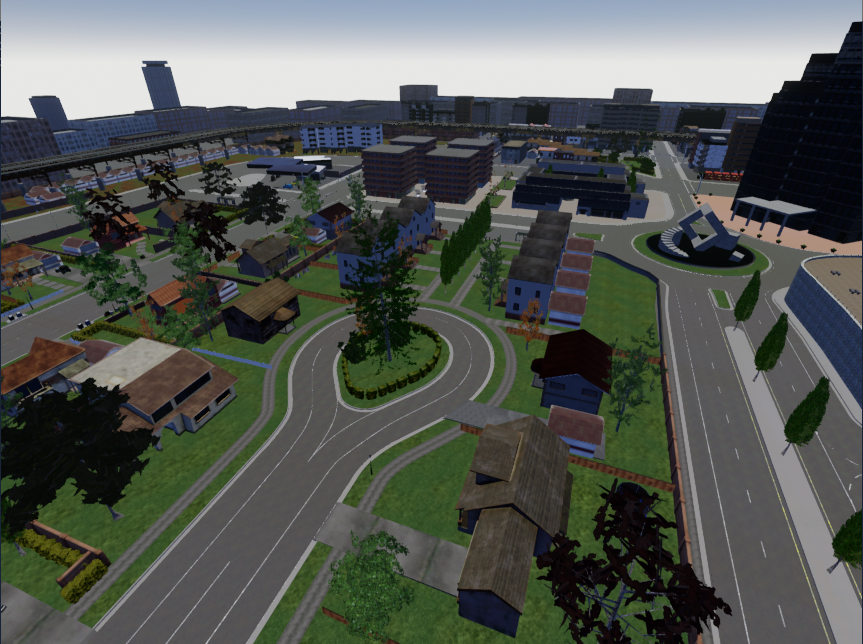
\includegraphics[scale=0.5]{images/carla_town03_example.png}
  \caption{Primjer mape pod nazivom Town03}
  \label{fig:town03_exmaple}
\end{figure}

Na slici \ref{fig:town03_exmaple} se vidi pogled na jedan od 7 mapa iz perspektive slobodne kamere. Korištene mape su definirane OpenDrive standardom. Simulator podržava raznolike senzore. Svi ti senzori se mogu postaviti samostalno na mapu, ali su najkorisniji kada se postave na drugo vozilo.

\subsection{Senzori}
\subsubsection{RGB senzor}
\begin{figure}[ht!]
  \centering
  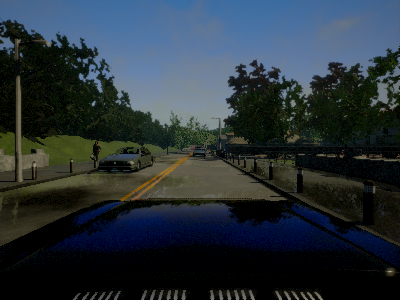
\includegraphics[scale=0.5]{images/rgb_example.png}
  \caption{Primjer regularne kamere}
  \label{fig:rgb_exmaple}
\end{figure}

RGB kamera je zapravo regularna kamera koja sliku onoga što vidi predstalja pomoću crvene, zelene i plave boje.

\subsubsection{Senzor dubine}
\begin{figure}[ht!]
  \centering
  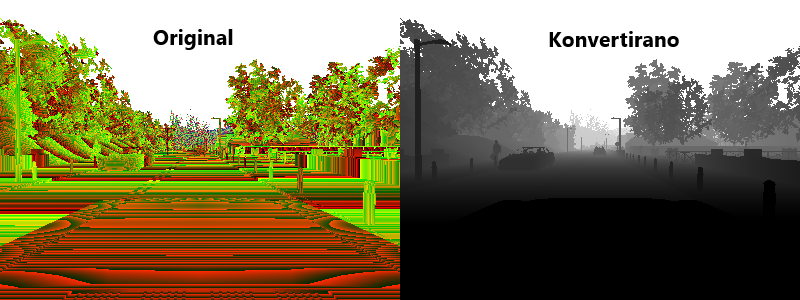
\includegraphics[scale=0.5]{images/depth_example.png}
  \caption{Primjer rezultata senzora dubine}
  \label{fig:depth_exmaple}
\end{figure}

Senzor dubine prikazuje svaki pixel na slici kamere u nijansama sive boje tj. ovisno koliko je objekt na određnome pixelu odaljen od kamere imat će svijetliju nijansu.

\newpage
\subsubsection{Senzor semantičke segmentacije}
\begin{figure}[ht!]
  \centering
  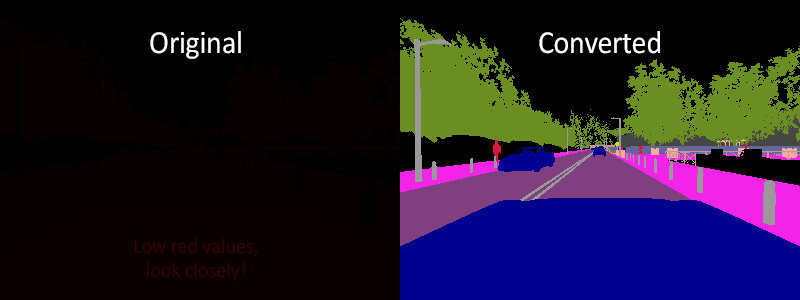
\includegraphics[scale=0.5]{images/sem_seg_exmaple.png}
  \caption{Primjer semantičke segmentacija}
  \label{fig:sem_seg_exmaple}
\end{figure}
Ovaj senzor dijeli sliku kamere na semantičke dijelove tj. objekterazličitog tima predstavlja drigim bojama. Na slici \ref{fig:sem_seg_exmaple} se vidi da je nebo crne boje, auti su plave boje, drveće je zeleno itd.

\subsubsection{LIDAR senzor}
\begin{figure}[ht!]
  \centering
  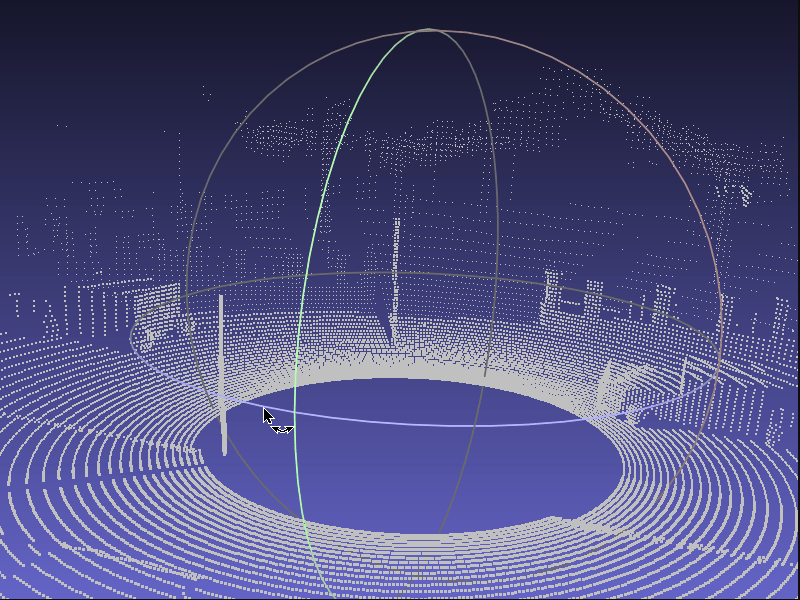
\includegraphics[scale=0.5]{images/LIDAR_examaple.png}
  \caption{LIDAr podaci}
  \label{fig:lidar_exmaple}
\end{figure}
LIDAR senzor je zapravo vertikalan skup lasera koji simuliraju skeniranje od 360 stupnjeva tako da se rotiraju određeni broj puta u sekundi. Povratni podaci senzora su zapravo točke do kojih su laseri uspjeli doći. Na slici \ref{fig:lidar_exmaple} se mogu vidjeti takvi podaci vizualizirani u programu MeshLab. Više o ulaznim parametrima senzora kasnije u radu.

\subsubsection{Senzor sudara}
Ovaj senzor dojavljuje klijentskome programu ako se vozila sudarilo s drugim objektom u simulaciji.

\subsubsection{Senzor prijelaza trake}
Ovaj senzor dojavljuje klijentskome programu ako je vozilo prošlo preko trake na cesti.

\subsubsection{GNSS senzor}
Senzor koji dojavljuje klijentskome programu trenutnu GNSS lokaciju vozila. Ta lokacija se interno računa tako da se lokacija vozila dodaje na geografsku referentnu lokaciju definiranu za cijelu mapu.

\subsubsection{Senzor prepreke}
Ovaj senzor javlja klijentskome programu ako se ispred vozila nalazi prepreka.

\subsection{Promet}
Postoji poveći broj već unaprijed definiranih vozila koja se mogu koristiti. Mogu se koristiti kao nositelji senzora ili kao ostali sudionici u prometu. Carla ima dobro definirana prometna pravila te semafore da bi simulacija izgledala što vjernije.